\subsection{Derivation of the Gradient Descent ODE}
We begin by considering the discrete-time gradient descent updates for the convex function $f$
\begin{align*}
    x_{k+1} = x_k - s \nabla f(x_k) 
\end{align*}
In order to derive the continuous-time limit of this equation, we simply rescale by $s$ and take $s \to 0$ making the \textit{ansatz} $x_k \approx X(ks)$ for some smooth curve $X(t)$ with the discrete/continuous scaling $t=ks$. Rescaling and rearranging gives
\begin{align}
    \frac{x_{k+1} - x_k}{s} = - \nabla f(x_k) \label{gd}
\end{align}
We then appeal to Taylor's theorem to approximate $x_{k+1} \approx X(t+s)$ as
\begin{align*}
    \frac{x_{k+1} - x_k}{s} = \dot{X}(t) + o(s)
\end{align*}
Combining with \eqref{gd} gives
\begin{align*}
    \dot{X}(t) + o(s) = - \nabla f(X)
\end{align*}
Matching terms at lowest order we obtain the continuous-time gradient flow
\begin{align}
    \dot{X}(t) = -\nabla f(X) \label{gdode}
\end{align}
Assuming the $f(X)$ has Lipschitz gradients the (local) existence and uniqueness of solutions to this ODE follows immediately from the Cauchy-Lipschitz theorem \citep{teschl2012ordinary}.
\subsection{Convergence Analysis}
\subsubsection{Weakly Convex Case}
Proving convergence of the solution trajectories of an ODE can often be achieved using an intuitive Lyapunov argument. In the simple case of gradient descent, considering the Lyapunov (or energy) function
\begin{align}
\label{gdlyap}
    V(X(t), t) = t (f(X(t)) - f(x^*)) + \frac{1}{2}||X(t)-x^*||^2
\end{align}
proves to be fruitful \citep{su2014differential}.

\begin{theorem}
The Lyapunov function
\begin{align*}
    V(X(t), t) = t (f(X(t)) - f(x^*)) + \frac{1}{2}||X(t)-x^*||^2
\end{align*}
satisfies $\dot{V}(X(t), t) \leq 0$ under the gradient flow $\dot{X}(t) = -\nabla f(X(t))$ and implies that:
\begin{align*}
    f(X(t)) - f(x^*) \leq \frac{||X(0)-x^*||_2^2}{2t}
\end{align*}
\end{theorem}

\proofstart
Here we assume that $x^*$ is the unique global minimizer of the convex function $f$. Direct computation shows that we have:
\begin{align*}
    \dot{V} &= f(X(t)) - f(x^*) + t \langle \nabla f(X(t)), \dot{X}(t) \rangle + \langle \dot{X}(t), X(t)-x^* \rangle \\
    &= \underbrace{f(X(t)) - f(x^*) - \langle \nabla f(X(t)), X(t) - x^* \rangle}_{\leq 0} \underbrace{- t || \nabla f(X(t))||_2^2}_{\leq 0} \\
    &\leq 0
\end{align*}
where by convexity we have that $f(X(t)) - f(x^*) - \langle \nabla f(X(t)), X(t) - x^* \rangle \leq 0$ and $ - t ||f(X(t))||_2^2 \leq 0$ since $t>0$. Now, using that $||X(t)-x^*||_2^2$ is non-negative, and that is $V$ is non-increasing function (since $\dot{V} \leq 0$) we immediately obtain that
\begin{align*}
    f(X(t)) - f(x^*) = \frac{V(X(t), t)}{t} - \frac{1}{2t} ||X(t) - x^*||_2^2 \leq \frac{V(X(t), t)}{t} \leq \frac{V(X(0), 0)}{t} = \frac{||X(0)-x^*||_2^2}{2t}
\end{align*}
which shows that $f(X(t)) \to f(x^*)$ at a $\mathcal{O}(1/t)$ convergence rate matching the $\mathcal{O}(1/k)$ convergence rate of gradient descent for convex, $\beta$-smooth functions \citep{DBLP:journals/ftml/Bubeck15}.
\proofend

\subsubsection{Strongly Convex Case}
To the best of our knowledge, there is not an explicit proof of the exponential convergence rate of the gradient descent ODE for strongly convex functions in the literature. Indeed, despite its simplicity, the first formal proof we found of the $O(1/t)$ convergence rate of the continuous-time gradient flow is in \citet{su2014differential}. We provide a Lyapunov function and proof of the exponential convergence rate of the gradient descent ODE, which will be a useful warm-up for analyzing the Nesterov (II) acceleration scheme applied to strongly convex functions.

\begin{theorem}
For an $\alpha$-strongly convex function the Lyapunov functional:
\begin{align*}
    V(X(t), t) = e^{\alpha t} \underbrace{\left[ f(X(t)) - f(x^*) + \frac{1}{2}||X(t)-x^*||^2 \right]}_{E(X(t), t)}
\end{align*}
satisfies $\dot{V}(X(t), t) \leq 0$ under the gradient flow $\dot{X}(t) = -\nabla f(X(t))$ implying that
\begin{align}
f(X(t)) - f(x^*) \leq e^{-\alpha t} (f(X(0))-f(x^*)+\frac{1}{2}(||X(0)-x^*||_2^2) \underbrace{\leq}_{\beta-\textit{smooth}} e^{-\alpha t} \left( \frac{\beta+1}{2} ||X(0) - x^*||_2^2 \right) 
\end{align}
\end{theorem}

\proofstart
Here $x^*$ is the unique global minimizer of the convex function $f$.
Direct computation shows that we have
\begin{align*}
    & \dot{V}(X(t), t) = \alpha e^{\alpha t} E(X(t), t) + e^{\alpha t} \dot{E}(X(t), t) \implies \\ 
    & \dot{V}(X(t), t) \leq 0 \iff \dot{E}(X(t), t) \leq -\alpha E(X(t), t)
\end{align*}
Recalling that the $\alpha$-strong convexity of $f$ implies $f(x^*) \geq f(X(t)) + \langle \nabla f(X(t)), x^*-X(t) \rangle + \alpha/2 ||x^*-X(t)||_2^2$ we can see that
\begin{align*}
    \dot{E}(X(t), t) &= \langle \nabla f(X(t)), \dot{X} \rangle + \langle X(t) - x^*, \dot{X}(t) \rangle \\
    &= - \langle \nabla  f(X(t)), \nabla f(X(t)) \rangle - \langle X(t) - x^*, \nabla f(X(t)) \rangle \\
    &= -||\nabla f(X(t))||_2^2 +\langle \nabla f(X(t)), x^*-X(t) \rangle \\
    &\leq -||\nabla f(X(t))||_2^2 - (f(X(t)) - f(x^*)) - \alpha/2 ||x^*-X(t)||_2^2\\
    &\leq -||\nabla f(X(t))||_2^2 - (f(X(t)) - f(x^*)) - \alpha/2 ||x^*-X(t)||_2^2 + \alpha E(X(t), t) - \alpha E(X(t), t) \\
    &\leq -||\nabla f(X(t))||_2^2 - (f(X(t)) - f(x^*)) + \alpha (f(X(t)) - f(x^*)) -\alpha E(X(t), t)
\end{align*}
We now appeal to the  Polyak-Lojasiewicz (PL) inequality -- $\frac{1}{2} ||\nabla f(x)||_2^2 \geq \alpha (f(x) - f(x^*))$ -- to complete the proof\footnote{The PL condition is weaker then strong convexity, but a simple argument shows that $\alpha$-strong convexity implies the $\alpha$-PL inequality.}. Interestingly, unlike the weakly convex case, we find it necessary to use the $-||\nabla f(X(t))||_2^2||$ to control the positive term $\alpha(f(X(t) - f(x^*))$.

Applying the $\alpha$-PL inequality gives that
\begin{align*}
    \dot{E}(X(t), t) &\leq -||\nabla f(X(t))||_2^2 - (f(X(t)) - f(x^*)) + \alpha (f(X(t)) - f(x^*)) -\alpha E(X(t), t) \\
    & \leq -2 \alpha (f(X(t)-f(x^*)) - (f(X(t)-f(x^*)) + \alpha (f(X(t)-f(x^*)) - \alpha E(X(t), t)) \\
    &\leq -(\alpha+1) (f(X(t)-f(x^*)) - \alpha E(X(t), t)\\
    &\leq -\alpha E(X(t), t)
\end{align*}

Now, using that $||X(t)-x^*||_2^2$ is non-negative, and that is $V$ is non-increasing function (since $\dot{V} \leq 0$) we immediately obtain:
\begin{align*}
    & f(X(t)) - f(x^*) = e^{-\alpha t} V(X(t), t) - \frac{1}{2} ||X(t) - x^*||_2^2 \leq e^{-\alpha t} V(X(t), t) \leq e^{-\alpha t} V(X(0), 0) = \\
    & e^{-\alpha t} (f(X(0))-f(x^*)+\frac{1}{2}(||X(0)-x^*||_2^2) \underbrace{\leq}_{\beta-\textit{smooth}} e^{-\alpha t} \left( \frac{\beta+1}{2} ||X(0) - x^*||_2^2 \right) 
\end{align*}
matching the exponential convergence rate of gradient descent applied to strongly convex functions.

\proofend

\subsection{Derivation of the Nesterov (I) ODE}
We now look to the continuous-time limit of the of the Nesterov (I) scheme analyzed in \citep{su2014differential}. Recalling the discrete-time Nesterov updates in \eqref{eq:nesterov1}
\begin{align*}
    x_k &= y_{k-1} - s \nabla f(y_{k-1})\\
    y_k &= x_k + \frac{k-1}{k+2} (x_k - x_{k-1})
\end{align*}
adding the $k+1$st update of $x_k$ as $x_{k+1} = y_k - s \nabla f(y_k)$ and the $k$th update of $y_k$ as $y_k = x_k + \frac{k-1}{k+2}(x_k-x_{k-1})$ gives
\begin{align}
    x_{k+1} - x_{k} = \frac{k-1}{k+2}(x_{k}-x_{k-1}) - s \nabla f(y_k) \label{diff1}
\end{align}
In order to derive the continuous-time limit of this set of equations, it is tempting to rescale this equation by $s$ and take $s \to 0$. However, this procedure will produce a degenerate limit as will become more apparent in the later derivation. As shown in \citet{su2014differential}, it is necessary to consider the \textit{ansatz} $x_k \approx X(k \sqrt{s})$ for some smooth curve $X(t)$, where the discrete/continuous time scaling takes the form $t = k \sqrt{s}$. That is we must rescale \eqref{diff1} by $\sqrt{s}$ to obtain
\begin{align}
    (x_{k+1} - x_{k})/\sqrt{s} = \left(\frac{k-1}{k+2}(x_{k}-x_{k-1}) \right)/\sqrt{s} - \sqrt{s} \nabla f(y_k) \label{diff2}
\end{align}
and take $s \to 0$ to obtain the correct limit. With this time-scaling we will have $X(t) \approx x_{t/\sqrt{s}} = x_k$ and $X(t+ \sqrt{s}) \approx x_{(t+\sqrt{s})/\sqrt{s}} = x_{k+1}$. With this ansatz we can appeal to Taylor's theorem to approximate
\begin{align*}
    (x_{k+1}-x_{k})/\sqrt{s} = \dot{X}(t) + \frac{1}{2} \ddot{X}(t) \sqrt{s} + o(\sqrt{s})
    \\
    (x_k - x_{k-1})/\sqrt{s} = \dot{X}(t) - \frac{1}{2}\ddot{X}(t) \sqrt{s} + o(\sqrt{s})
\end{align*}
and similarly that
\begin{align*}
    \sqrt{s} \nabla f(y_k) &= \sqrt{s} \nabla f(X(t)) + o(\sqrt{s})
    \\
    \frac{k-1}{k+2} &= 1 - \frac{3}{k+2} \approx 1 - \frac{3}{k} = 1 - \frac{3 \sqrt{s}}{t}
\end{align*}
where we have used the fact that $y_k - X(t) = o(1)$ in the first equality and noted that taking $s \to 0$ implies $k$ is ``large" for any non-zero $t$ in the second inequality.
Combining these approximations with \eqref{diff2} equation gives
\begin{align*}
    \dot{X}(t) + \frac{1}{2} \ddot{X}(t) \sqrt{s} + o(\sqrt{s}) = (1 - 3\frac{\sqrt{s}}{t} + o(\sqrt{s})(\dot{X}(t) - \frac{1}{2} \ddot{X}(t) \sqrt{s} + o(\sqrt{s})) - \sqrt{s} \nabla f(X(t)) + o(\sqrt{s})
\end{align*}
Matching terms at lowest order -- in particular at order $\sqrt{s}$ -- we obtain:
\begin{align}
    \ddot{X} + \frac{3}{t} \dot{X} + \nabla f(X) = 0 \label{ode}
\end{align}
The first initial condition is simply $X(0) = x_0$. Taking $k=1$ in \eqref{diff2} yields $(x_2-x_1)/\sqrt{s} = \sqrt{s} \nabla f(y_1) = o(1)$. Thus, to match terms at lowest order, we must take $\dot{X}(0)=0$. Note that, had we considered this derivation with the prospective time-scaling $t=ks$ instead of $t = k\sqrt{s}$ we would have obtained a degenerate limit in which the $\dot{X}, \ddot{X}$ were at $o(s)$ in the expansion while the $\nabla f(X)$ term would be at $o(1)$.

\begin{figure}[!h]
\begin{center}
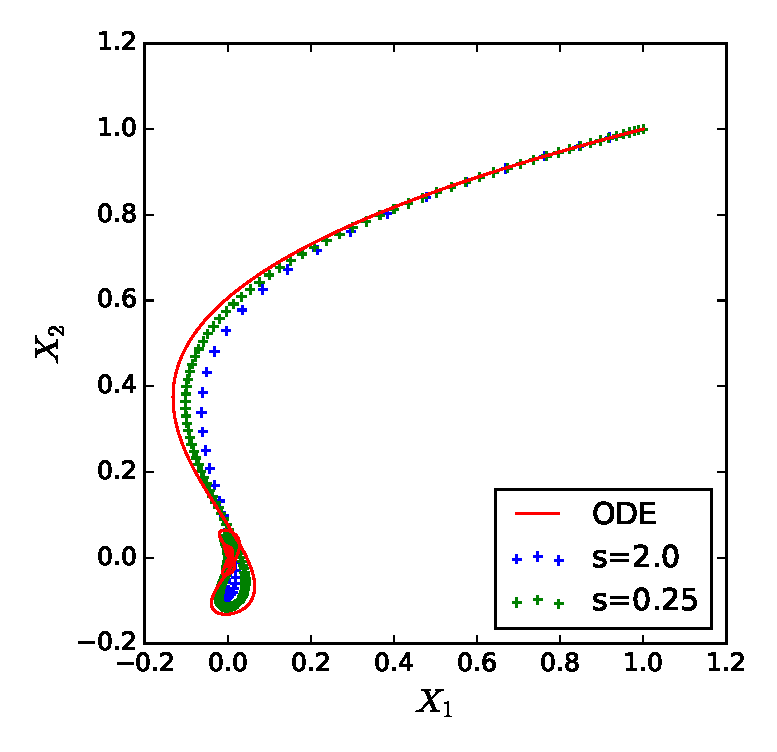
\includegraphics[width=0.5\linewidth]{Experiments/quadratic_traj_compare_annealed.eps}
\caption{Comparison of the ODE trajectories $X(t)$ with the discrete-time Nesterov updates for minimizing $f(x) = .02 X_1^2 + 0.005 X_2^2$.}
\end{center}
\end{figure}

\begin{figure}[!h]
\begin{center}
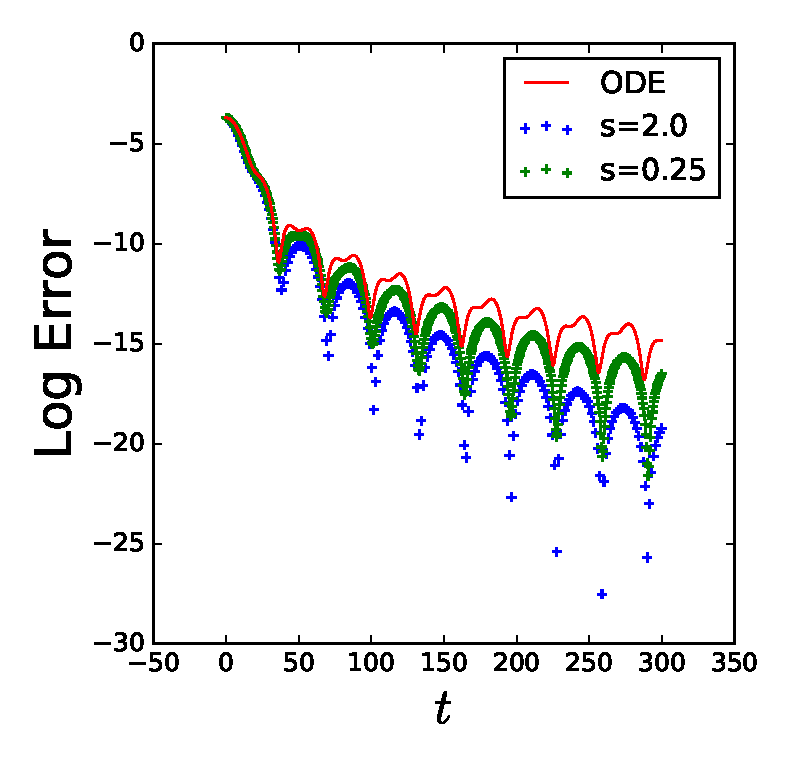
\includegraphics[width=0.5\linewidth]{Experiments/quadratic_errors_compare_annealed.eps}
\caption{Comparison of the errors of the ODE trajectories $X(t)$ with the discrete-time Nesterov updates for minimizing $f(x) = .02 X_1^2 + 0.005 X_2^2$.}
\end{center}
\end{figure}

Classical ODE theory unfortunately does not imply the (local) existence and uniqueness to this ODE since the coefficient $\frac{3}{t}$ is singular at $t=0$. However, as shown in \citet{su2014differential} the ODE is nonetheless well-posed. \citet{su2014differential} shows this by constructing a series of ODE's approximating \eqref{ode} by truncating $\frac{3}{t} = \frac{3}{\min \{ k, t \}}$ for a sequence of $k\to 0$. One then can use a compactness argument to extract a convergent subsequence by appealing to the Arzela-Ascoli theorem whose limit is the well-defined solution to \eqref{ode}.

This intuitive derivation is formally correct as the following theorem shown in \citet{su2014differential} justifies:
\begin{theorem}
    For any function $L$-Lipschitz function as the step-size $s \to 0$ the sequence of $x_k$ satisfying the discrete-time updates of \eqref{eq:nesterov1} converges to the solution of the ODE \eqref{ode} in the sense that: \\
    \begin{align*}
    \lim_{s \to 0} \max_{0 \leq k \leq \frac{T}{\sqrt{s}}} ||x_k-X(k\sqrt{s})|| = 0
    \end{align*}
\end{theorem}

\subsubsection{Convergence Analysis}
Analogous to the case of gradient descent, a simply Lyapunov argument can be used to show the convergence of the Nesterov ODE to the minimizer of $f$ in continuous-time in stark contrast to the complicated discrete-time proof convergence proof of the Nesterov (I) scheme \citep{su2014differential}.  

\begin{theorem}
The Lyapunov function
\begin{align*}
    V(t) = t^2 (f(X(t)) - f^*) + 2||X+t \dot{X}/2 - x^*||_2^2
\end{align*}
satisfies $\dot{V}(X(t), t) \leq 0$ under the flow of the Nesterov (I) ODE in \eqref{ode} implying that 
\begin{align*}
    f(X(t)) - f(x^*) \leq \frac{2 ||X(0)-x^*||_2^2}{t^2}
\end{align*}
\end{theorem}

\proofstart
We assume $x^*$ is the unique minimizer of $f$. By direct computation we have that
\begin{align*}
    \dot{V} = 2t(f(X(t)) - f(x^*)) + t^2 \langle \nabla f(X(t)), \dot{X} \rangle + 4 \langle X + \frac{t}{2} \dot{X} - x^*, \frac{3}{2} \dot{X} + \frac{t}{2} \ddot{X} \rangle
\end{align*}
Substituting $3 \dot{X}/2 + t \ddot{X}/2$ with $-t \nabla f(X)/2$ gives
\begin{align*}
    \dot{V} = 2t(f(X(t)) - f(x^*)) + 4\langle X(t)-x^*, -t \nabla f(X(t))/2 \rangle = 2t \left( f(X(t)) - f(x^*) - \langle X(t)-x^*, \nabla f(X(t)) \rangle \right ) \leq 0
\end{align*}
where by convexity we have that $f(X(t)) - f(x^*) - \langle \nabla f(X(t)), X(t) - x^* \rangle \leq 0$. Now, using that $||X+t \dot{X}/2 - x^*||_2^2$ is non-negative, and that is $V$ is non-increasing function (since $\dot{V} \leq 0$) we immediately obtain that
\begin{align*}
    f(X(t)) - f(x^*) &= \frac{V(X(t), t)}{t^2} - \frac{2}{t^2} ||X+t \dot{X}/2 - x^*||_2^2 \\
    &\leq  \frac{V(X(t), t)}{t^2}\leq \frac{V(X(0), 0)}{t^2} = \frac{2 ||X(0)-x^*||_2^2}{t^2}
\end{align*}
which shows that $f(X(t)) \to f(x^*)$ at a $\mathcal{O}(1/t^2)$ convergence rate matching the $\mathcal{O}(1/k^2)$ convergence rate of the Nesterov (I) scheme for weakly convex functions.
\proofend

\subsubsection{The ``Magic" Constant 3}
Recall the constant $3$ appearing in the Nesterov ODE \eqref{ode}
\begin{align}
    \ddot{X} + \frac{3}{t} \dot{X} + \nabla f(X) 
\end{align}
originates from the $\frac{k-1}{k+2} = 1 - \frac{3}{k} + \mathcal{O}(1/k^2)$ in \eqref{eq:nesterov1}, and controls the strength of the ``damping" term in the dynamics. The continuous-time perspective shows that this choice of constant is not haphazard -- in fact the constant $3$ can be replaced with any larger number $r>3$ while preserving the the $\mathcal{O}(1/t^2)$ convergence rate. However, smaller choices of $r$ quickly lead to oscillatority, non-convergent solutions \citep{su2014differential}.
\begin{figure}[H]
\begin{center}
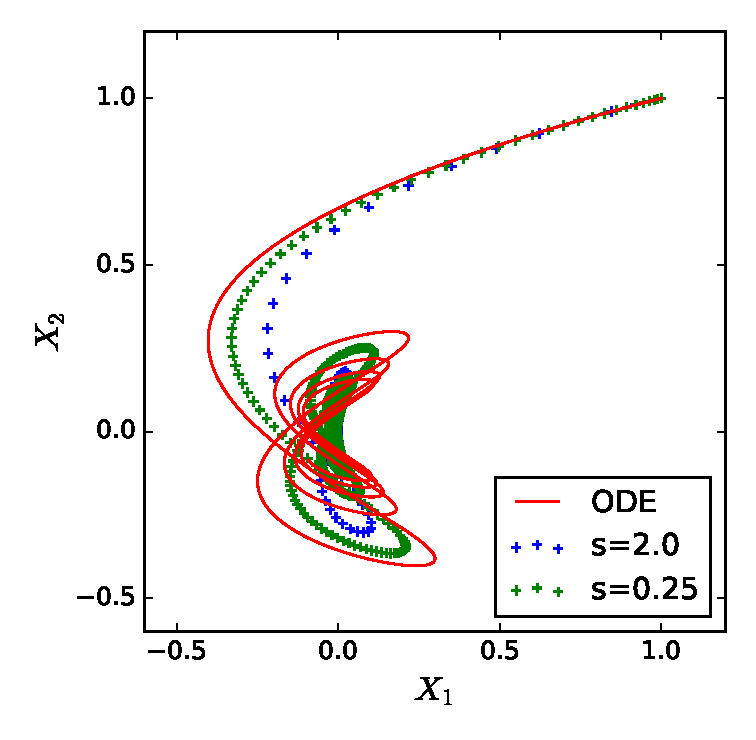
\includegraphics[width=0.5\linewidth]{Experiments/quadratic_traj_compare_annealed_r1.eps}
\caption{Non-convergent trajectories of ODE and Nesterov (I) scheme $X(t)$ (with $r=1$) when minimizing $f(x) = .02 X_1^2 + 0.005 X_2^2$.}
\end{center}
\end{figure}

\
If we consider
\begin{align}
    \ddot{X} + \frac{r}{t} \dot{X} + \nabla f(X) \label{highfrictionode}
\end{align}
with initial conditions $X(0) = x_0$ and $\dot{X}(0) = 0$ for $r>3$, this ODE possesses a stronger ``friction" term than \eqref{ode}. As before the convergence rate can be proven by constructing an appropriate energy functional.
\begin{theorem}
The Lyapunov functional (defined for $r>3$)
\begin{align}
\label{agdode}
    V(X(t), t) = \frac{2t^2}{r-1} \left( f(X(t)) -f(x^*) \right) + (r-1) ||X(t) + \frac{t}{r-1}\dot{X}(t) -x^*||_2^2
\end{align}
satisfies $\dot{V}(X(t), t) \leq 0$ under the flow of \eqref{highfrictionode} and implies that
\begin{align*}
    f(X(t)) - f(x^*) \leq \frac{(r-1)^2 ||X(0)-x^*||_2^2}{2 t^2}
\end{align*}
\end{theorem}
\proofstart
Direct computation gives that
\begin{align*}
    \dot{V}(X(t), t)) = \frac{4t}{r-1}(f(X(t)) - f(x^*)) + \frac{2t^2}{r-1} \langle \nabla f, \dot{X} \rangle + 2 \langle X + \frac{t}{r-1} \dot{X} - x^*, r \dot{X} + t \ddot{X} \rangle
\end{align*}
Using $r\dot{X} + t \ddot{X} = -t \nabla f(X(t))$ yields
\begin{align*}
    \dot{V}(X(t), t)) = \frac{4t}{r-1} (f(X(t) - f(x^*)) - 2t \langle X(t) - x^*, \nabla f(X(t)) \rangle \leq - \frac{2(r-3)t}{r-1}(f(X(t))-f(x^*))
\end{align*}
where the last inequality follows from the convexity of $f$ which gives: $-\langle X(t) - x^*, \nabla f(X(t)) \rangle \leq f(X(t)) - f(x^*)$. Since the $f(X(t)) - f(x^*) \geq 0$ this implies $\dot{V}$ is non-decreasing\footnote{The $r-3$ term in the convexity bound on $\dot{V}$ also provides some intuition for the role of the ``magic" constant $3$.}. Since the term $(r-1) ||X(t) + \frac{t}{r-1} \dot{X}(t) - x^*||_2^2$ is non-negative and $V(t)$ is non-decreasing we obtain a $\mathcal{O}(1/t^2)$ convergence rate as before
\begin{align*}
    f(X(t)) - f(x^*) &= \frac{r-1}{2t^2} V(X(t), t) - \frac{(r-1)^2}{2t^2} ||X(t) + \frac{t}{r-1} \dot{X}(t) - x^*||_2^2 \\
    &\leq \frac{r-1}{2t^2} V(X(t), t) \\
    &\leq \frac{r-1}{2t^2} V(X(0), 0) = \frac{(r-1)^2 ||X(0)-x^*||_2^2}{2 t^2}
\end{align*}
\proofend

As in \citet{su2014differential} we can empirically validate the advantages of a stronger friction term by generalizing the Nesterov (I) scheme in discrete-time, using our insights from continuous-time, to include a stronger ``friction" term
\begin{align}
\begin{split}
    x_k &= y_{k-1} - s \nabla f(y_{k-1})\\
    y_k &= x_k + \frac{k-1}{k+r-1} (x_k - x_{k-1}) \label{nesterov_r}
\end{split}
\end{align}
in our discrete-time updates. We consider the performance of this scheme on three synthetic examples (taking $s=\frac{1}{\beta}$ in each) inspired by 3 simple machine learning problems:

\begin{itemize}
\item \textbf{Least Squares}: $f(x) = \frac{1}{2} || Ax - b||^2$ where $A \in \mathbb{R}^{100 \times 500}$ with $A_{ij} \sim \mathcal{N}(0,1)$ and $b \in \mathbb{R}^{100}$ with $b \sim \mathcal{N}(0,9)$ entries.
\item \textbf{Lasso with Fat Design}: $f(x) = \frac{1}{2} ||Ax - b||^2 + \lambda |x|_1$ where $A, b$ are defined as before and $\lambda = 4$.
\item \textbf{Logistic Regression}: $f(x) = \sum_{i=1}^n -y_i b_i^\top x + \log(1+ \exp(b_i^\top x))$ with $B = (b_1, \cdots, b_n)^T \in \mathbb{R}^{500 \times 100}$ and $B_{ij} \sim \mathcal{N}(0,1)$ i.i.d. The labels $y_i \in \{0,1\}$ are generated using the logistic map $\mathbb{P}(Y_i=1) = \frac{1}{1+\exp(-a_i^\top x^0)}$ with $x^0 \sim \mathcal{N}(0,\frac{1}{100})$.
\end{itemize}

\begin{figure}[!htb]
\minipage{0.32\textwidth}
  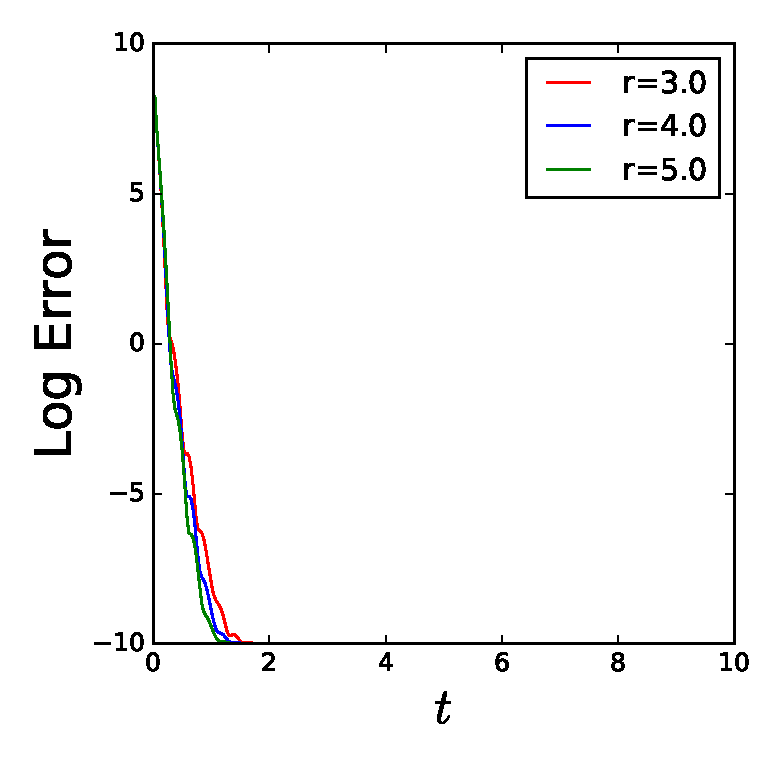
\includegraphics[width=1\linewidth]{SourceFiles/plots/least_squares_errors_compare.eps}
\caption{Error of $f-f^*$ vs iteration number for the Least Squares objective with increasing values of $r$.}
\label{fig: Rerrors1}
\endminipage\hfill
\minipage{0.32\textwidth}
  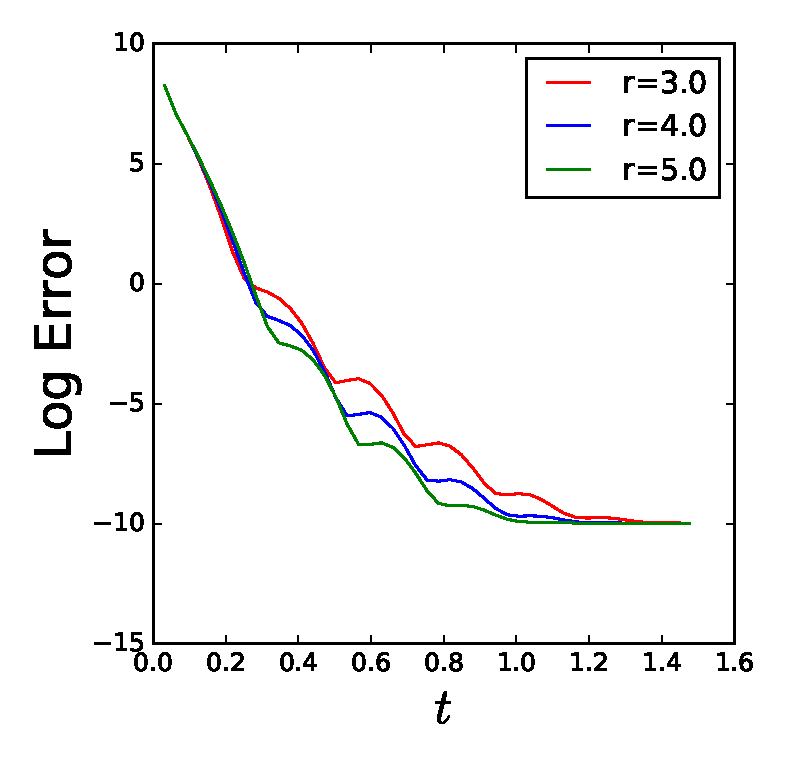
\includegraphics[width=1\linewidth]{SourceFiles/plots/lasso_fat_design_errors_compare.eps}
\caption{Error of $f-f^*$ vs iteration number for the Lasso objective with increasing values of $r$.}
\label{fig: Rerrors2}
\endminipage\hfill
\minipage{0.32\textwidth}%
 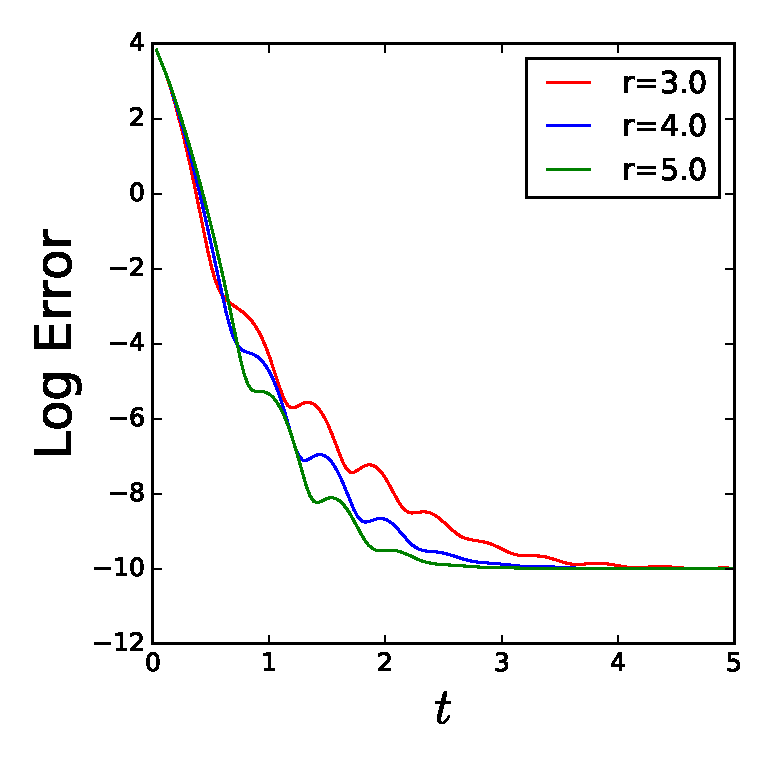
\includegraphics[width=1\linewidth]{SourceFiles/plots/logistic_regression_errors_compare.eps}
\caption{Error of $f-f^*$ vs iteration number for the Logistic Regression objective with increasing values of $r$.}
\label{fig: Rerrors3}
\endminipage
\end{figure}

As we can see in Figure \ref{fig: Rerrors1}, \ref{fig: Rerrors2}, and \ref{fig: Rerrors3} increasing the strength of the friction term correspondingly increases the rate of convergence of the generalized Nesterov (I) scheme to the global optima as observed in \cite{su2014differential}.
 
\section{Derivation of the Nesterov (II) ODE}
In the original work of \citet{ nesterov2004introductory} two acceleration methods are presented in discrete-time. We refer to ``time-varying" case for $\beta$-smooth functions -- \eqref{eq:nesterov1} which accelerates the $\mathcal{O}(1/k)$ rate of gradient descent to an optimal $\mathcal{O}(1/k^2)$ rate -- as the Nesterov (I) scheme. \citet{ nesterov2004introductory} also presented an optimal algorithm for $\alpha$-strongly convex, $\beta$-smooth functions achieving an optimal geometric convergence rate $\mathcal{O} \left (\exp(-\frac{k}{\sqrt{\kappa}}) \right)$ compared to the $\mathcal{O} \left (\exp(-\frac{k}{\kappa}) \right)$ of gradient descent
\begin{align}
    & x_{k} = y_{k-1} - \underbrace{\frac{1}{\beta}}_{s} \nabla f(y_{k-1}) \label{eq:constantnesterov1} \\
    & y_{k} = x_{k} + \left( \frac{\sqrt{\kappa}-1}{\sqrt{\kappa}+1} \right) \left( x_{k} - x_{k-1} \right)  \label{eq:constantnesterov2}
\end{align}
 The work of \citet{su2014differential} does not derive a continuous-time limit of this Nesterov (II) scheme with fixed momentum coefficient. We provide such a derivation here -- in particular showing the continuous-time limit maps onto the dynamics of critically damped oscillator. This connection reveals the choice of momentum coefficient is far from arbitrary. In particular, if $f$ is quadratic, it is a well-known result from classical mechanics that critical damping leads to the fastest relaxation of the continuous-time dynamical system.

 
 In order to obtain the desired it is crucial to note that in \eqref{eq:constantnesterov2} we have that $s = \frac{1}{\beta}$ and $\kappa = \frac{\beta}{\alpha} = \frac{1}{\alpha s}$ -- so $\kappa$ is implicitly dependent on $s$ since $s$ is coupled to the smoothness of the function $f$\footnote{For a fixed function $f$ that is $\beta$ smooth, it is somewhat odd to evaluate the limit $s \to 0 \implies \beta \to \infty$. However, this is scaling is crucial to achieve the desired limit -- further it is still consistent since if $\beta_2 > \beta_1$ then $\beta_1$--smoothness implies $\beta_2$--smoothness.}. We first add the $k+1$st term of \eqref{eq:constantnesterov1} -- $x_{k+1} = y_k - s \nabla f(y_k)$ to the $k$th update of \eqref{eq:constantnesterov2} -- $y_k = x_k + \frac{\sqrt{\kappa}-1}{\sqrt{\kappa}+1} (x_k - x_{k-1})$ to obtain
 \begin{align*}
     x_{k+1} = x_{k} + \frac{\sqrt{\kappa}-1}{\sqrt{\kappa}+1}(x_{k}-x_{k-1}) - s \nabla f(y_k)
 \end{align*}

 In order to derive the continuous-time limit of this set of equations, we rescale this equation by $\sqrt{s}$ and take $s \to 0$ as in the derivation of \eqref{ode}. In particular we consider the \textit{ansatz} $x_k \approx X(k \sqrt{s})$ for some smooth curve $X(t)$, where the discrete/continuous time scaling takes the form $t = k \sqrt{s}$.
 \begin{align*}
    \frac{x_{k+1}-x_k}{\sqrt{s}} = \frac{\sqrt{\kappa(s)}-1}{\sqrt{\kappa(s)}+1} \left( \frac{x_{k}-x_{k-1}}{\sqrt{s}} \right) - \sqrt{s} \nabla f(y_k) \implies \\
    \frac{(x_{k+1}-x_k)-(x_{k}-x_{k-1})}{\sqrt{s}} = (\frac{\sqrt{\kappa(s)}-1}{\sqrt{\kappa(s)}+1}-1) \left( \frac{x_{k}-x_{k-1}}{\sqrt{s}} \right) - \sqrt{s} \nabla f(y_k)
 \end{align*}
 
 We will approximate $x_{k+1} \approx X(t+\sqrt{s})$, $x_k \approx X(t)$, $x_{k-1} \approx X(t-\sqrt{s})$.
 Thus we have that
 \begin{align*}
     \frac{x_{k+1} - x_k}{\sqrt{s}} &= \dot{X}(t) + \frac{1}{2} \sqrt{s} \ddot{X} o(\sqrt{s}) \\
     \frac{x_k - x_{k-1}}{\sqrt{s}} &= \dot{X}(t) + \frac{1}{2} \sqrt{s} \ddot{X} o(\sqrt{s}) \\
     \nabla f(y_k) &= \nabla f(X(t)) + o(1) \\
    \frac{\sqrt{\kappa(s)}-1}{\sqrt{\kappa(s)}+1}-1 &= -\frac{2}{\sqrt{\kappa}+1} = -\frac{2}{\frac{1}{\sqrt{\alpha s}}+1} = -\frac{2 \sqrt{\alpha s}}{1+\sqrt{\alpha s}} = -2 \sqrt{\alpha} \sqrt{s} (1+o(\sqrt{s}))
 \end{align*}
 which gives
 \begin{align*}
     \sqrt{s} \ddot{X} + o(s) = (2 \sqrt{\alpha} \sqrt{s} + o(s))(\sqrt{s} \dot{X} + o(1)) - \sqrt{s} \nabla f(X(t))
 \end{align*}
 Matching terms at lowest-order yields the desired ODE as
 \begin{align}
     \ddot{X}(t) + 2 \sqrt{\alpha} \dot{X} + \nabla f(X(t)) = 0. \label{constantnesterovode}
 \end{align}
As in the case of the Nesterov (I) ODE we can easily show from \eqref{eq:constantnesterov2} that the appropriate initial conditions for \eqref{constantnesterovode} are $X(0) = x_0$ and $\dot{X}(0)=0$.

Assuming the $f(X)$ has Lipschitz gradients the (local) existence and uniqueness of solutions to this ODE follows immediately from the Cauchy-Lipschitz theorem \citep{teschl2012ordinary}. We find, studying this ODE in the case of quadratic $f$ is particularly fruitful since this ODE is a linear differential equation and maps exactly onto the physics of a damped harmonic oscillator.

\subsection{Analysis for Quadratic $f(X) = \alpha X^2$ }

We can extract further insight into the Nesterov acceleration (II) scheme by studying it's continuous-time limit in \eqref{constantnesterovode} when $f(X)$ is quadratic. Crucially, when $f(X) = \alpha X^2$, the differential equation \eqref{constantnesterovode} is \textit{linear} and hence admits an explicit, analytic solution. 

In particular, if we consider\footnote{Note that the limit of the Nesterov acceleration (II) scheme of \eqref{eq:constantnesterov1} which yields \eqref{constantnesterovode} corresponds to taking $\zeta=1$. in this parametrization.}
\begin{align*}
   \underbrace{\ddot{X}}_{\text{``mass"}} + \underbrace{2 \zeta \sqrt{\alpha} \dot{X}}_{\text{``damping"}} + \underbrace{\alpha X}_{\text{``force"}} = 0
\end{align*}
the ODE maps \textit{precisely} onto the dynamics of the damped, simple harmonic oscillator from classical mechanics \citep{morin2008introduction}. The solutions follows immediately from the theory of ordinary differential equations \citep{morin2008introduction}.  
\begin{align*}
   X(t) = \begin{cases}
   & e^{-\zeta \sqrt{\alpha} t} \left( C \cos(\alpha(1-\zeta^2) t+\phi \right) \text{ when } \zeta < 1 \ \textcolor{green}{\text{Under Damping}}  \\
   & e^{-\zeta \sqrt{\alpha} t}(A+B t) \text{ when } \zeta = 1 \ \textcolor{red}{\text{Critical Damping}} \\
   & A e^{-\sqrt{\alpha}(\zeta - \sqrt{\zeta^2-1})) t}+ B e^{ -(\sqrt{\alpha}(\zeta + \sqrt{\zeta^2-1}) t})   \text{ when } \zeta > 1 \ \textcolor{blue}{\text{Over Damping}} 
   \end{cases}
\end{align*}

\begin{figure}[!h]
\begin{center}
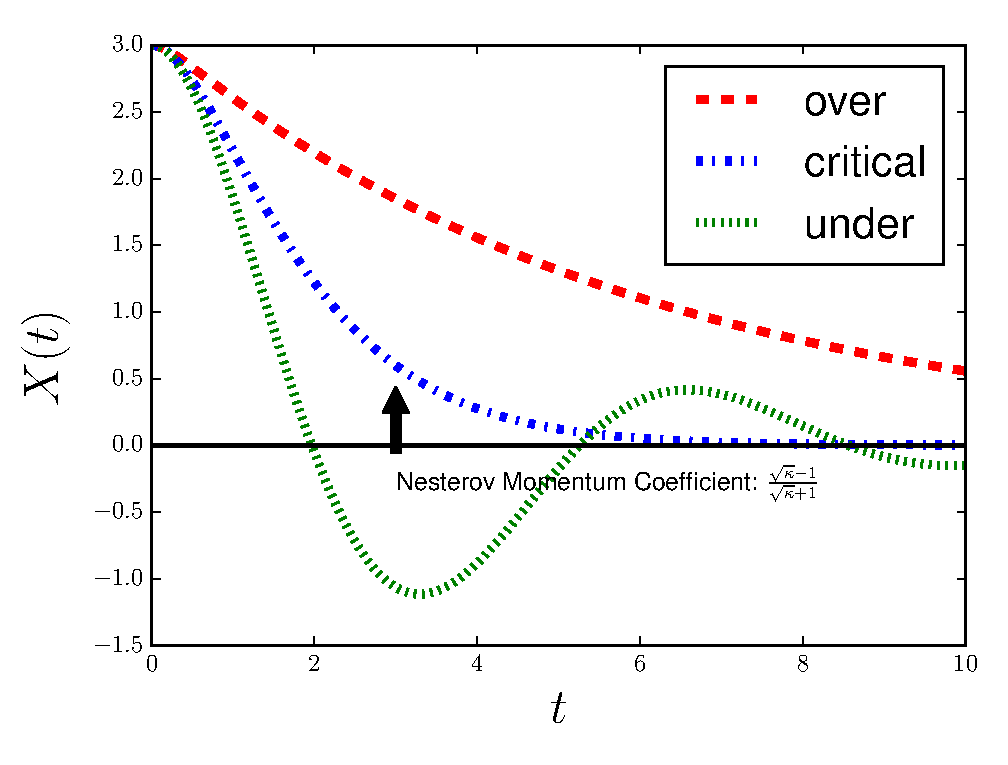
\includegraphics[width=0.6\linewidth]{Experiments/critical_damp_Nesterov.eps}
\caption{Comparison of the $X(t)$ for $X(0)=3$, $\dot{X}(0)=0$ for $\zeta > 1$, $\zeta=1$, and $\zeta < 1$.}
\end{center}
\end{figure}

Asymptotically as $t \to \infty$ we have that $X(t)$ slowest decaying mode scales as
\begin{align*}
   X(t) \sim \begin{cases}
   & e^{-\sqrt{\alpha} \zeta t}\text{ when } \zeta < 1 \ \textcolor{green}{\text{Under Damping}} \\
   & e^{-\sqrt{\alpha} \zeta t + \log t} \text{ when } \zeta = 1 \ \textcolor{red}{\text{Critical Damping}} \\
   & e^{-\sqrt{\alpha}(\zeta - \sqrt{\zeta^2-1})) t}  \text{ when } \zeta > 1 \ \textcolor{blue}{\text{Over Damping}} 
   \end{cases}
\end{align*}

Importantly, up to logarithmic factors, we have that the amplitude of $X(t)$ decays \textit{fastest in the critically damped case} since we have that both
\begin{align*}
    & \zeta < 1 \text{ when } \zeta \text{ is under-damped,} \\
    & \zeta -\sqrt{\zeta^2-1} < 1 \text{ when } \zeta  \text{ is over-damped.}
\end{align*}
Indeed it is a well-known result in classical mechanics that choosing $\zeta=1$ leads to the fastest dissipation of mechanical energy from a damped harmonic oscillator. This is a critical design principle used in many real systems -- such as shock absorbers -- where one would like to have the system reach equilibrium as quick as possible (without overshooting and oscillating -- underdamping or moving too slowly -- overdamping).

Thus, we find that the particular choice of the Nesterov ``momentum" coefficient $\frac{\sqrt{\kappa}-1}{\sqrt{\kappa}+1}$ is far from arbitrary, algebraic trick. Rather, the choice of of the Nesterov momentum \textit{is} critically damping its continuous-time limit (when $f(x)$ is quadratic).

\subsection{Convergence Analysis}
We can also construct the Lyapunov functional to prove an exponential convergence rate for the continuous-time Nesterov (II) ODE.
\begin{theorem}
The Lyapunov functional
\begin{align*}
    V(X(t), t) = e^{\sqrt{\alpha} t} \underbrace{\left [f(X(t)) - f(x^*) + \frac{\alpha}{2}||x^*-X(t)-\frac{1}{\sqrt{\alpha}} \dot{X}(t)||_2^2 \right]}_{E(X(t), t)}
\end{align*}
satisfies $\dot{V}(X(t), t)$ under the flow of the Nesterov (II) ODE in \eqref{constantnesterovode} implying that
\begin{align*}
    f(X(t)) - f(x^*) \leq e^{-\sqrt{\alpha}t} \left(f(X(0))-f(x^*)+\frac{\alpha}{2}||x^*-X(0)||_2^2 \right) \underbrace{\leq}_{\beta-smooth} e^{-\sqrt{\alpha}t} \left(\frac{\alpha+\beta}{2}||x^*-X(0)||_2^2 \right)
\end{align*}
\end{theorem}
\proofstart
Here $x^*$ is the unique global minimizer of the convex function $f$. Direct computation gives
\begin{align*}
    & \dot{V}(X(t), t) = \sqrt{\alpha} e^{\sqrt{\alpha} t} E(X(t), t) + e^{\sqrt{\alpha} t} \dot{E}(X(t), t) \implies \\ 
    & \dot{V}(X(t), t) \leq 0 \iff \dot{E}(X(t), t) \leq -\sqrt{\alpha} E(X(t), t)
\end{align*}
Thus we obtain that
\begin{align*}
    & \dot{E}(X(t), t) = \langle \nabla f(X(t)), \dot{X} \rangle + \langle x^* - X(t) - \frac{1}{\sqrt{\alpha}} \dot{X}(t), - \dot{X}(t) - \frac{1}{\sqrt{\alpha}} \ddot{X}(t) \rangle
\end{align*}
Using $-\frac{1}{\sqrt{\alpha}} \ddot{X}(t) = 2 \dot{X}(t) + \frac{1}{\sqrt{\alpha}} \nabla f(X(t))$ gives
\begin{align*}
    \dot{E}(X(t), t) &= \langle \nabla  f(X(t)), \dot{X}(t) \rangle + \alpha \langle x^* - X(t) - \frac{1}{\sqrt{\alpha}} \dot{X}(t), \dot{X}(t) + \frac{1}{\sqrt{\alpha}} \nabla f(X(t)) \rangle\\ &= \sqrt{\alpha} \langle \nabla f(X(t)), x^* - X(t) \rangle +
    \alpha \langle x^* - X(t) - \frac{1}{\sqrt{\alpha}} \dot{X}(t), \dot{X}(t) \rangle 
\end{align*}
Now, using $\alpha$-strong convexity of $f$, $f(x^*) \geq f(X(t)) + \langle \nabla f(X(t)), x^*-X(t) \rangle + \alpha/2 ||x^*-X(t)||_2^2$, and
\begin{align*}
    \dot{E}(X(t), t) &\leq -\sqrt{\alpha} ( f(X(t)) - f(x^*) + \frac{\alpha}{2} ||x^*-X(t)||_2^2) + \alpha \langle x^*-X(t)-\frac{1}{\sqrt{\alpha}} \dot{X}(t), \dot{X}(t) \rangle\\ 
    &= -\sqrt{\alpha} ( f(X(t)) - f(x^*) + \frac{\alpha}{2} ||x^*-X(t)-\frac{1}{\sqrt{\alpha}} \dot{X}(t) ||_2^2 \\
    &\qquad +\sqrt{\alpha} \langle x^*-X(t), \dot{X}(t) \rangle -\frac{1}{2} ||X(t)||_2^2)  + \alpha \langle x^*-X(t)-\frac{1}{\sqrt{\alpha}} \dot{X}(t), \dot{X}(t) \rangle \\
    & = -\sqrt{\alpha} E(X(t), t) - \sqrt{\alpha} \langle x^*-X(t)-\frac{1}{\sqrt{\alpha}} \dot{X}(t), \dot{X}(t) \rangle\\ & \qquad-\frac{1}{2} ||\dot{X}(t)||_2^2 + \alpha \langle x^*-X(t)-\frac{1}{\sqrt{\alpha}} \dot{X}(t), \dot{X}(t) \rangle \\
    & = -\sqrt{\alpha} E(X(t), t) - \frac{1}{2} ||\dot{X}(t)||_2^2 \\
    & \leq -\sqrt{\alpha} E(X(t), t)
\end{align*}
as desired. The Lyapunov functional gives:
\begin{align*}
    f(X(t)) - f(x^*) &= e^{-\sqrt{\alpha}t} V(X(t), t) - \frac{\alpha}{2} ||x^*-X(t)-\frac{1}{\sqrt{\alpha}} \dot{X}(t)||_2^2 \\
    & = e^{-\sqrt{\alpha}t} V(X(t), t) \leq e^{-\sqrt{\alpha}t} V(X(0), 0)  \\
    & = e^{-\sqrt{\alpha}t} \left(f(X(0))-f(x^*)+\frac{\alpha}{2}||x^*-X(0)||_2^2 \right) \\
    & \underbrace{\leq}_{\beta-smooth} e^{-\sqrt{\alpha}t} \left(\frac{\alpha+\beta}{2}||x^*-X(0)||_2^2 \right)
\end{align*}
matching the exponential convergence rate of the discrete-time Nesterov (II) scheme.
\proofend 
 
 \begin{comment}
 \subsection{$\kappa$ does not scale with $s$}

 We first add the $k+1$st term of \eqref{eq:constantnesterov1} -- $x_{k+1} = y_k - s \nabla f(y_k)$ to the $k$th update of \eqref{eq:constantnesterov2} -- $y_k = x_k + \frac{\sqrt{\kappa}-1}{\sqrt{\kappa}+1} (x_k - x_{k-1})$ to obtain:
 \begin{align*}
     x_{k+1} = x_{k} + \frac{\sqrt{\kappa}-1}{\sqrt{\kappa}+1}(x_{k}-x_{k-1}) - s \nabla f(y_k)
 \end{align*}
 In order to derive the continuous-time limit of this set of equations, we might initially consider rescaling this equation by $\sqrt{s}$ and take $s \to 0$ as in the derivation of \eqref{ode}. However, this procedure produces a degenerate limit. Instead we rescale by $s$ as in the case of the continuous-time limit of gradient descent in \eqref{gdode}. In particular we consider the \textit{ansatz} $x_k \approx X(k s)$ for some smooth curve $X(t)$, where the discrete/continuous time scaling takes the form $t = k s$.
 \begin{align*}
    \frac{x_{k+1}-x_k}{s} = \frac{\sqrt{\kappa}-1}{\sqrt{\kappa}+1} \left( \frac{x_{k}-x_{k-1}}{s} \right) - \nabla f(y_k)
 \end{align*}
 
 We will approximate $x_{k+1} \approx X(t+s)$, $x_k \approx X(t)$, $x_{k-1} \approx X(t-s)$. So rescaling b
 Thus we have that:
 \begin{align*}
     & \frac{x_{k+1} - x_k}{s} = \dot{X}(t) + o(1) \\
     & \frac{x_k - x_{k-1}}{s} = \dot{X}(t) + o(1) \\
     & \nabla f(y_k) = \nabla f(X(t)) + o(1)
 \end{align*}
 which gives:
 \begin{align*}
     \dot{X}(t) + o(1) = \frac{\sqrt{\kappa}-1}{\sqrt{\kappa}+1} \left( \dot{X}(t) + o(1)\right) - \nabla f(X(t)) + o(1)
 \end{align*}
 Matching terms at lowest-order yields the desired ODE as:
 \begin{align}
     \dot{X}(t) = -\frac{\sqrt{\kappa}+1}{2} \nabla f(X(t)) \label{constantnesterovode}
 \end{align}
The condition number for a convex function will always be $\kappa > 1 \implies \frac{\sqrt{\kappa}+1}{2} > 1$. Relative to the gradient descent ODE \eqref{gdode}, the ``constant" acceleration ODE \eqref{constantnesterovode} has a forcing term with increased constant coefficient. Intuitively, this suggests this ODE will converge to equilibrium faster.

We can construct a Lyapunov functional for analogous to the case of gradient descent:
\begin{align*}
    V(X(t), t) = \frac{\sqrt{\kappa}+1}{2}t(f(X(t)) - f(x^*)) + \frac{1}{2}||X(t)-x^*||^2
\end{align*}
Direct computation shows that we have:
\begin{align*}
    & \dot{V}= \frac{\sqrt{\kappa}+1}{2}(f(X(t)) - f(x^*)) + \frac{\sqrt{\kappa}+1}{2} t \langle \nabla f(X(t)), \dot{X}(t) \rangle + \langle \dot{X}(t), X(t)-x^* \rangle = \\
    & \frac{\sqrt{\kappa}+1}{2} \underbrace{f(X(t)) - f(x^*) - \langle \nabla f(X(t)), X(t) - x^* \rangle}_{\leq 0} \underbrace{- t (\frac{\sqrt{\kappa}+1}{2})^2 || \nabla f(X(t))||_2^2}_{\leq 0} \implies \\
    & \dot{V} \leq 0
\end{align*}
where by convexity we have that $f(X(t)) - f(x^*) - \langle \nabla f(X(t)), X(t) - x^* \rangle \leq 0$ and $ - t ||f(X(t))||_2^2 \leq 0$ since $t>0$. Now, using that $||X(t)-x^*||_2^2$ is non-negative, and that is $V$ is non-increasing function (since $\dot{V} \leq 0$) we immediately obtain that:
\begin{align*}
    & f(X(t)) - f(x^*) = \frac{2}{\sqrt{\kappa}+1} \frac{V(X(t), t)}{t} - \frac{1}{(\sqrt{\kappa}+1)t} ||X(t) - x^*||_2^2 \leq \frac{2}{\sqrt{\kappa}+1} \frac{V(X(t), t)}{t} \leq \frac{2}{\sqrt{\kappa}+1} \frac{V(X(0), 0)}{t} = \\ & \frac{2}{\sqrt{\kappa}+1} \frac{||X(0)-x^*||_2^2}{2t}
\end{align*}

Since $\frac{2}{\sqrt{\kappa}+1} < 1$ this bound on the error is tighter than in the case of gradient descent.
\end{comment}









